Having separated private and social influences in individual agents, we next ask whether improving one agent's private evidence can redirect a collective trajectory, and how the effect changes with population size.

\textbf{Agent-level causal tracing via crop patching.} Activation patching measures how replacing selected internal activations changes an outcome \citep{meng2022locating,zhang2024patching}. We apply the intervention logic at the level of an agent's private input. Using a saved Germany crop layout selected from wrong-answer examples, a patch replaces one agent's original crop with a more informative crop of the same flag before initialization and on subsequent model calls. All other crops, the communication protocol, and the directed communication schedule are held fixed within the comparison; model responses are sampled afresh. Memory evolves through the usual interactions. Thus the intervention tests the collective effect of changing private visual evidence, rather than replacing hidden activations or directly setting an agent's belief.

\textbf{Selecting an intervention site.} We first patch each of the eight agent sites separately with the same informative crop, using one run per site and a common communication schedule (Fig.~\ref{fig:crop-patching}b). Three original-crop controls each have 25\% collective mean accuracy after ten rounds. Patching A4 yields the largest observed improvement, reaching 100\%, so we select A4 for repeated-run follow-up. The donor is an existing crop assigned to A1 in the saved layout; patching A1 is therefore an identity control. This screen identifies a useful intervention site in this setting, rather than a universal ranking of agents. As an isolated visual check, ten independent judgments of A4's original crop all identify Yemen, while ten judgments of the informative crop all identify Germany (\(N=1\) in panel d).

\textbf{Tracing collective correction.} Panels a and c show a selected pair of \(N=8\) runs with the same original layout and communication schedule. At the displayed endpoint, the original-crop run has two Germany answers and six Yemen answers (25\% collective mean accuracy); patching A4 produces eight Germany answers (100\%). The arrows connect country switches to matching recent messages, showing candidate transmission paths through the population. They are not separate interventions on those messages, so they do not establish the causal effect of each edge. The crop intervention is causal at the input level; the arrow map supplies a descriptive account of the ensuing exchanges. The displayed pair is included in the repeated-run results below.

\begin{figure*}[t]
    \centering
    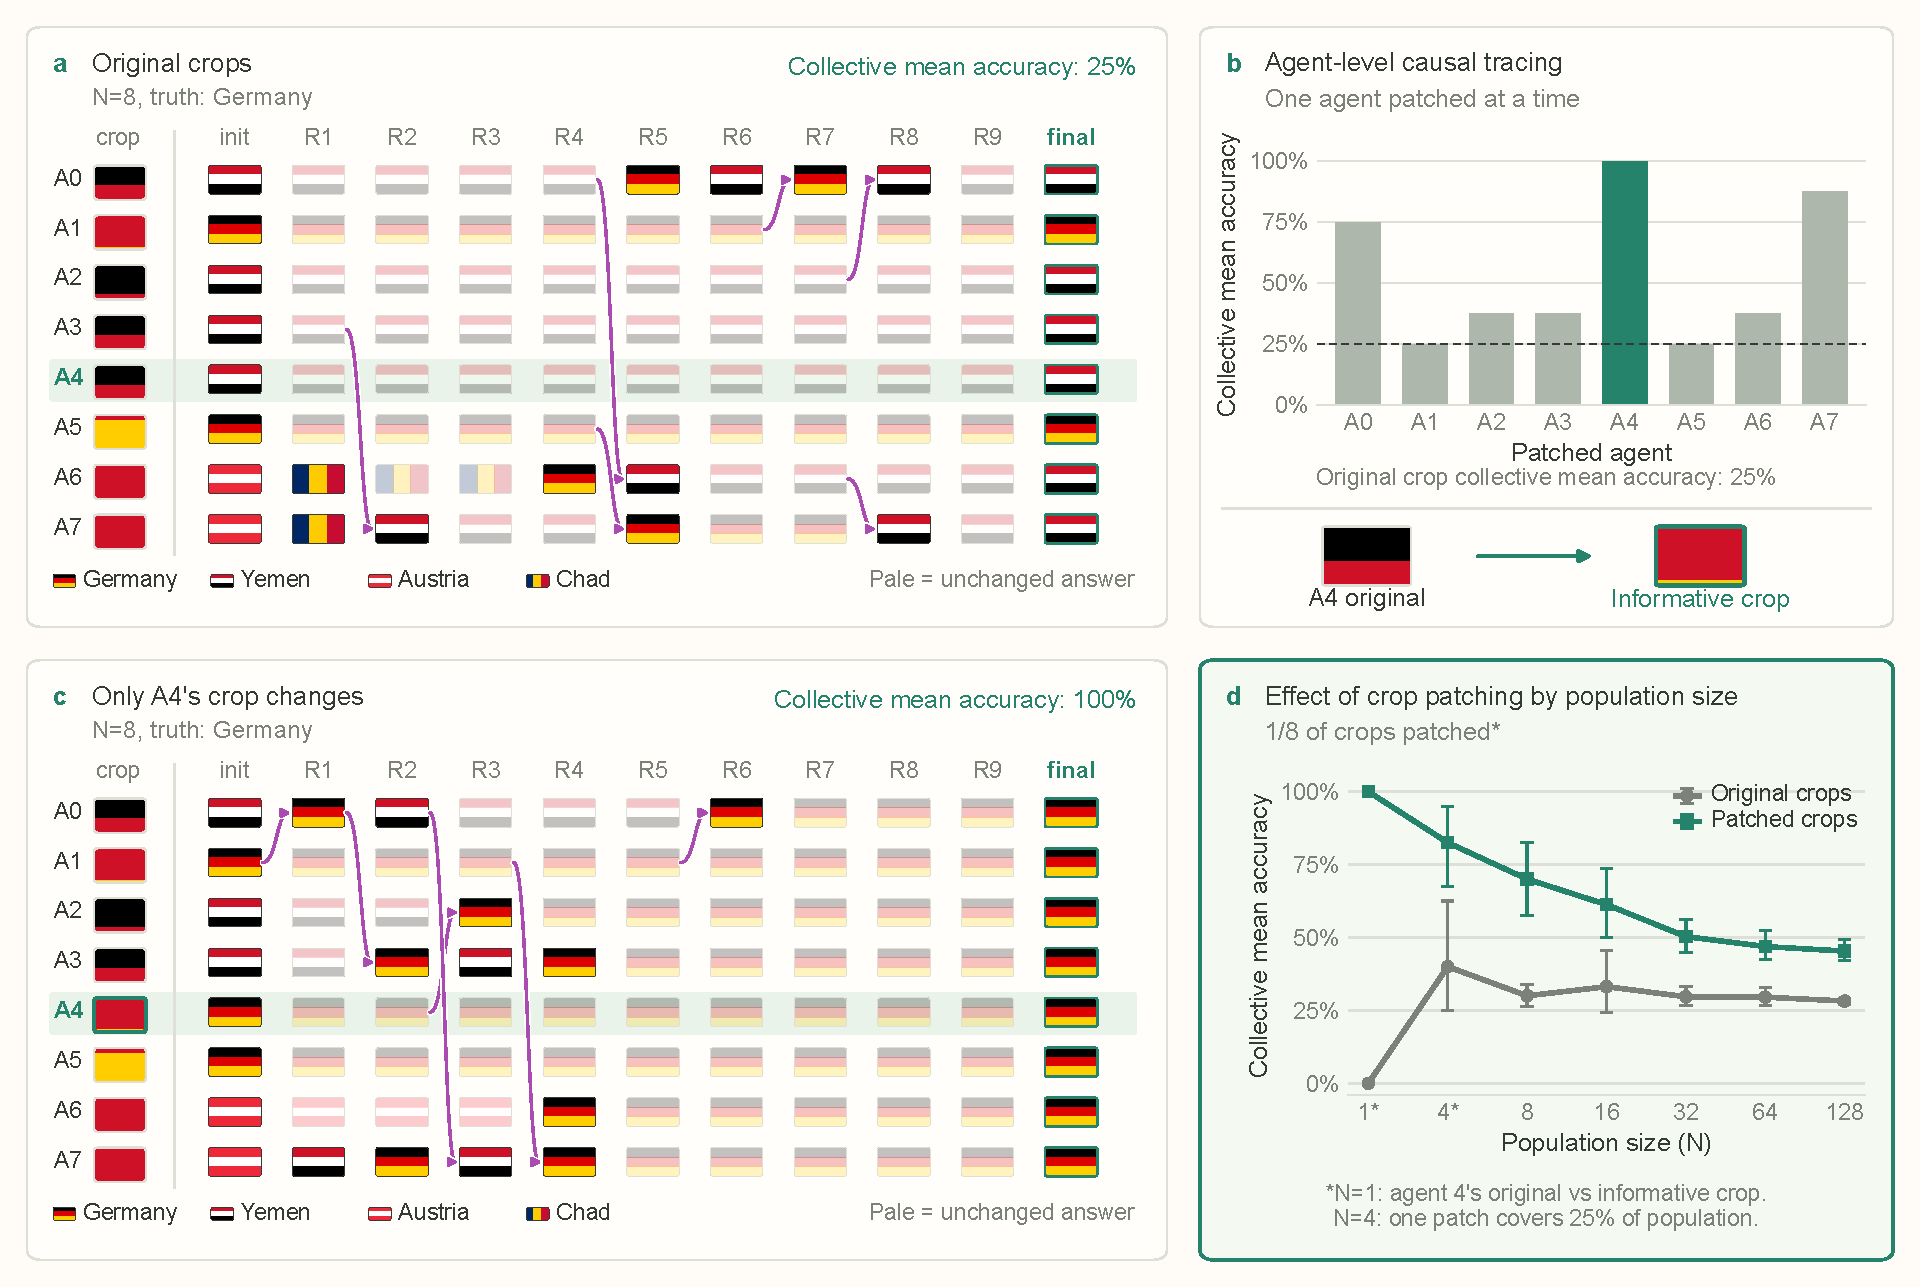
\includegraphics[width=\textwidth]{visuals/crop_patching_germany.pdf}
    \caption{\textbf{Agent-level crop patching and its collective effect.}
GPT-4o agents identify Germany from private crops and pairwise messages.
\textbf{(a,c)} A selected pair of \(N=8\) runs shares the crop layout and communication schedule; only A4's crop changes in c. Rows represent agents and flags their reported countries; faded flags mark unchanged answers. ``Final'' is round 10, yielding 25\% and 100\% collective mean accuracy. An arrow requires a recipient to switch country and its latest valid incoming message within that round to agree with both the sender's preceding-round answer and the recipient's new answer. These are message-compatible switches, not individually isolated causal effects.
\textbf{(b)} One separate run per intervention site, evaluated after ten rounds. The horizontal reference is the mean of three original-crop controls (25\% each). A4 has the largest observed improvement and is selected for follow-up. Its original and informative crops appear below; the donor is A1's existing crop, making the A1 condition an identity control.
\textbf{(d)} Original versus patched collective mean accuracy after ten rounds, with ten runs per condition at \(N\geq4\). A round contains \(N\) directed messages. For \(N=8\)--128, the same eight-crop layout is repeated, and one A4 copy per block of eight is patched (12.5\%). \(N=1\) instead uses ten independent isolated judgments per crop, with empty memory and no communication; patching its only crop changes 100\% of the population. \(N=4\) uses source crops A0, A1, A2, and A4, patching source A4 (25\% of the population); this subset was selected after examining six layouts. Population sizes occupy equally spaced categorical positions. Error bars are 95\% percentile bootstrap confidence intervals over whole runs (isolated judgments at \(N=1\)). The selected trace pair and its endpoint were chosen retrospectively; the pair also contributes to the ten-run \(N=8\) means. The trace, site screen, and population averages are distinct comparisons. Thus the \(N=1\) and \(N=4\) points are reference cases with different evidence compositions or intervention fractions, not a matched continuation of the \(N\geq8\) size comparison.}
    \label{fig:crop-patching}
\end{figure*}

\textbf{Patching effect across population sizes.} For each population size \(N\geq4\), we next evaluate the selected intervention over ten runs per condition, matching communication schedules between original and patched conditions. For \(N=8,16,32,64,128\), we repeat the same eight-crop layout and patch every copy of A4, keeping the intervention fraction at \(1/8\). For these social games, panel d compares collective mean accuracy after ten rounds; its vertical difference is the \emph{patching effect} on this outcome. At \(N=8\), collective mean accuracy rises from 30.0\% to 70.0\%, a 40.0 percentage-point effect (95\% paired bootstrap interval: 28.75--51.25 points). At \(N=128\), it rises from 28.2\% to 45.3\%, a 17.1-point effect (13.75--21.17 points). Improving the same fraction of private inputs therefore produces less collective correction at larger populations in this setup, while retaining a positive effect. The selected 25\% to 100\% trace illustrates a possible trajectory; it is not the repeated-run mean.

\textbf{Connecting interventions to the population theory.} The Germany comparison complements the evidence-coverage mechanism in Sec.~\ref{sec:stat-mech}, but tests a different population change. The theory samples independent crops as \(N\) increases, allowing previously absent evidence types to appear. The patching comparison at \(N\geq8\) instead fixes the empirical crop proportions by repetition. Its size dependence therefore concerns collective dynamics at a fixed interaction budget per agent, rather than the discovery of additional crop types. At fixed evidence fractions, Eq.~\eqref{eq:meanfield} has no explicit \(N\) dependence; explaining the measured change in patching effect requires analysis of finite-population dynamics or a richer update model. We do not fit that response here. The \(N=1\) and \(N=4\) reference cases also change the intervention fraction, so the complete curve should not be read as a size-only test of the theory's accuracy peak.

\textbf{Complementary approaches.} Causal interventions and statistical mechanics address different explanatory levels. An intervention asks how a specified change to private or social evidence affects behavior; a population model asks how evidence distributions and interaction rules generate drift, consensus, and polarization \citep{castellano2009statistical}. Patching results depend on the tested inputs, intervention sites, and outcome metric, and need not identify a unique or minimal mechanism \citep{zhang2024patching,heimersheim2024patching}. Here, crop patching establishes a context-dependent collective effect of private evidence, while the message traces identify candidate paths for further intervention. The smaller effect at larger \(N\) motivates examining population-level reinforcement alongside agent-level perturbations. It does not establish that causal tracing becomes impossible, or that mechanistic techniques cease to work.
